\item In \figref{fig:figure2345}, $PQ$ is a chord of length $8 cm$ of a circle of radius $5 cm$ and centre $\vec{O}$. The tangents at $P$ and $Q$ intersect at point $T$. Find the length of $TP$.
\begin{figure}[H]                                             \centering
         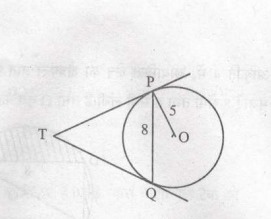
\includegraphics[width=\columnwidth]{figs/i2.jpeg}
			\caption{triangle45}
			\label{fig:figure2345}

                \end{figure}
\item Find the area of the segment shown in \figref{fig:figure5456}, if radius of the circle is $21 cm$ and $\angle AOB = 120\degree$ Use $\brak{n =\frac{22}{7}} $
\begin{figure}[H]                                     
\centering
	
 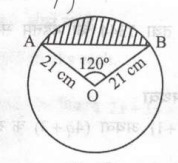
\includegraphics[width=\columnwidth]{figs/img123.jpeg}
		
\caption{circles45}
		
\label{fig:figure5456}
\end{figure}
\item In \figref{fig:figure6978}, a circle is inscribed in a $\triangle ABC$ having sides $BC=8 cm$, $AB = 10cm$ and $AC = 12 cm$. Find the lengths $BL$, $CM$ and $AN$.
                                         
\begin{figure}[H]                                     
\centering
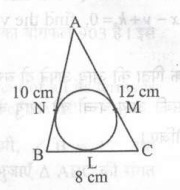
\includegraphics[width=\columnwidth]{figs/img234.jpeg}
\caption{circles45}
\label{fig:figure6978}

 \end{figure}
\end{enumerate}
